%==============================================================================
% Sjabloon poster bachelorproef
%==============================================================================
% Gebaseerd op document class `a0poster' door Gerlinde Kettl en Matthias Weiser
% Aangepast voor gebruik aan HOGENT door Jens Buysse en Bert Van Vreckem

\documentclass[a0,portrait]{hogent-poster}

% Info over de opleiding
\course{Bachelorproef}
\studyprogramme{toegepaste informatica}
\academicyear{2022-2023}
\institution{Hogeschool Gent, Valentin Vaerwyckweg 1, 9000 Gent}

% Info over de bachelorproef
\title{Kan containertechnologie gebruikt worden om de gecombineerde installatie van Hadoop, Spark en Kafka te automatiseren ?}
%\subtitle{Ondertitel (eventueel)}
\author{Jurn De Vleeschauwer}
\email{jurn.devleeschauwer@student.hogent.be}
\supervisor{Stijn Lievens}
\cosupervisor{Martijn Saelens} %(Bedrijf)}

% Indien ingevuld, wordt deze informatie toegevoegd aan het einde van de
% abstract. Zet in commentaar als je dit niet wilt.
\specialisation{Mobile \& Enterprise developer}
\keywords{Systeembeheer, Container, Big Data}
\projectrepo{https://github.com/jurnDeVleeschau/BP}

\begin{document}

\maketitle

\begin{abstract}
Container technologie wint de laatste jaren steeds meer aan belang. Het zou een goede oplossing kunnen zijn voor de installatie van applicaties gebruikt door studenten bij het vak “Big Data Processing”. De aspecten security en stabiliteit verdienen hierbij extra aandacht.
\end{abstract}

\begin{multicols}{2} % This is how many columns your poster will be broken into, a portrait poster is generally split into 2 columns

\section{Introductie}
In het kader van de opleiding Toegepaste Informatica HoGent gebruiken de studenten de Big Data frameworks Hadoop, Spark en Kafka zowel tijdens de les als tijdens de examens. Hiervoor worden deze applicaties op de laptop van de student geïnstalleerd, en daarmee gaat kostbare (leer)tijd verloren. Is het een mogelijkheid om deze software op de infrastructuur van het VIC te plaatsen, zodat dit geen tijd meer kost aan de student, en zou container technologie daarbij een rol kunnen spelen ?
\newline
\newline
Het beoogde resultaat van deze bachelorproef is meer inzicht te verschaffen in het gebruik van container technologie, toegepast op  installaties van Hadoop, Spark en Kafka en te komen tot aanbevelingen voor de installatie op het VIC\footnote{HOGENT Virtual IT Company}. Daarbij worden een aantal proof-of-concepts uitgevoerd om meer inzicht te krijgen in de complexiteit hiervan.

\section{Experimenten}
Op basis van de aandachtspunten rond security en stabiliteit, wat zich vooral vertaald in volledige afscherming van de gebruikers (studenten) van elkaar, en de mogelijkheden van container technologie, is er gekozen om een aparte omgeving per student te onderzoeken als mogelijke oplossing.
\newline
\newline
Een eerste experiment is het lokaal opzetten van Hadoop, Spark en Kafka met Docker, om inzicht te krijgen in de werking van container technologie en te komen tot een werkende Docker-Compose configuratie.
\newline
\newline


\begin{center}
  \captionsetup{type=figure}
  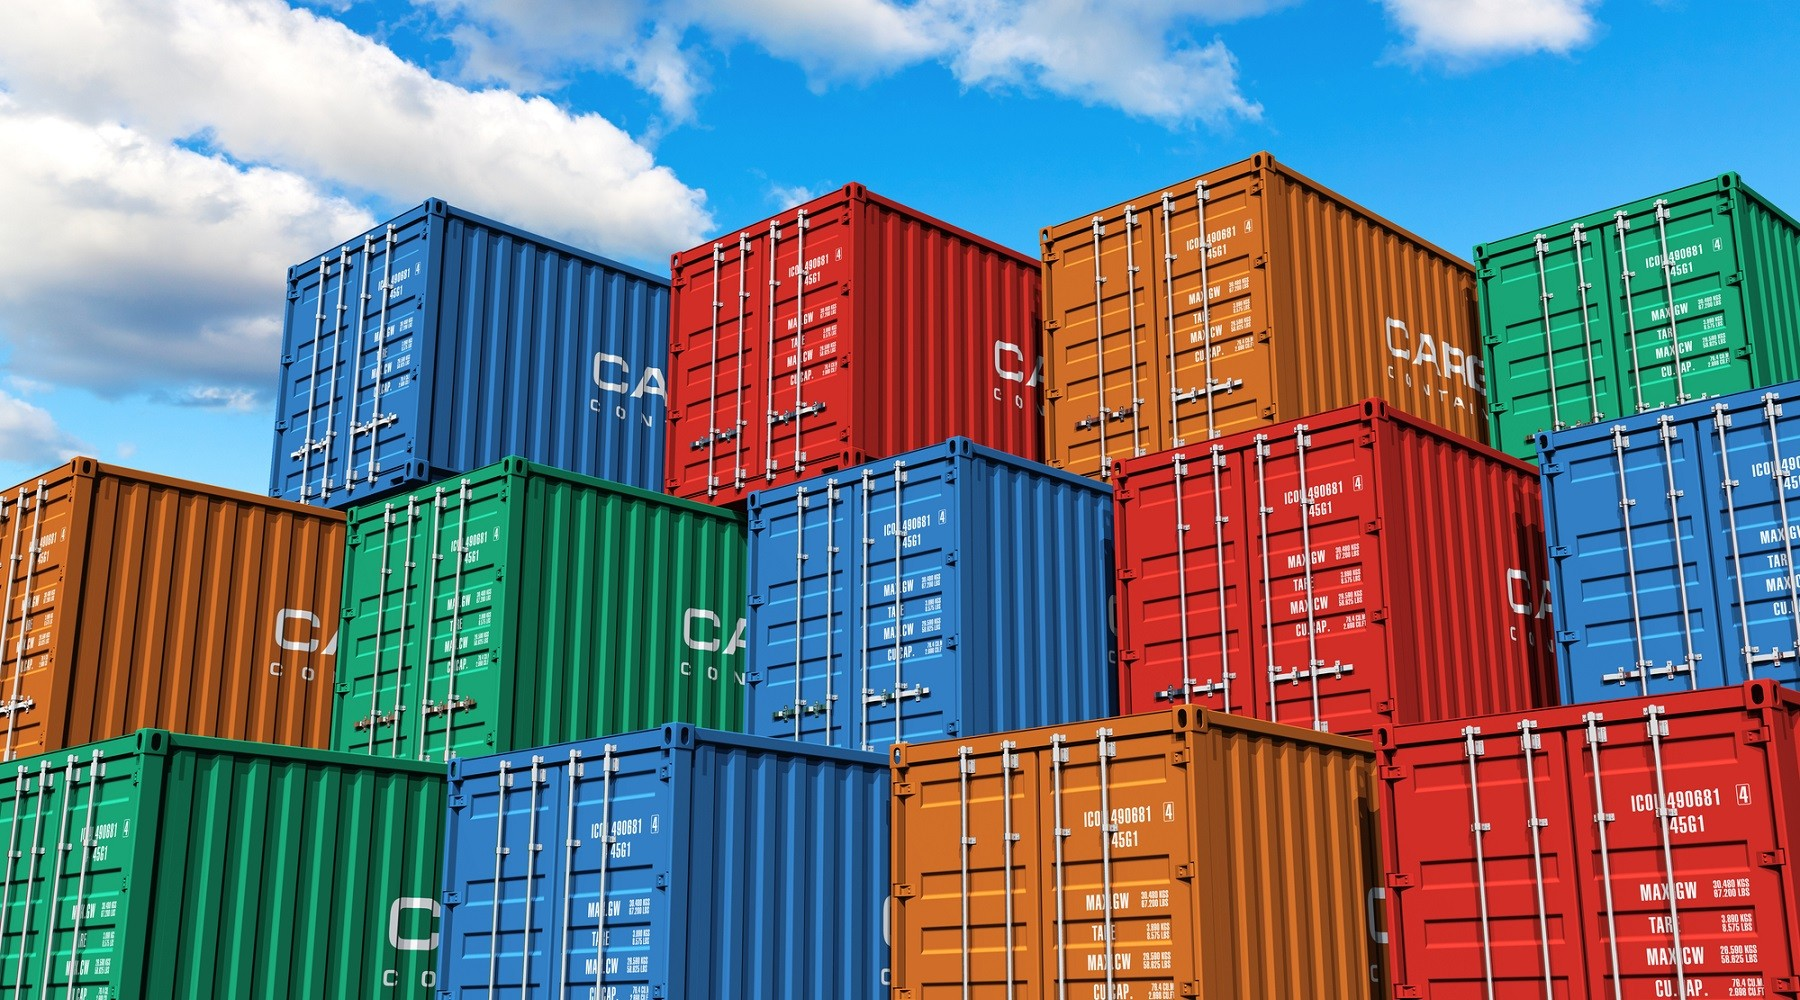
\includegraphics[width=1.0\linewidth]{containers.jpg}
  \captionof{figure}{Containers in de cloud}
\end{center}

\noindent In een tweede experiment werd dit omgezet naar een configuratie met Kubernetes, een veelgebruikte oplossing voor het beheer van containers, en omdat dit op termijn een mogelijkheid is voor het VIC.
\newline
\newline
In een derde experiment werd hieraan security toegevoegd, om elke omgeving volledig af te schermen van andere studenten door middel van authenticatie.
\newline
\newline


\section{Conclusies}
Uit de literatuurstudie blijkt dat container technologie meer en meer gebruikt wordt zowel in eigen data centers, zoals het VIC, als in publieke cloud omgevingen. De belangrijkste redenen hiervoor zijn het gemak en de stabiliteit van voorverpakte applicaties die zich snel laten installeren, de vlotte horizontale schaalbaarheid die zich vertaald in het eenvoudig toevoegen van extra containers, en de strikte afscheiding van containers die op eenzelfde machine draaien terwijl er hiervoor minder resources worden gebruikt dan voor virtuele machines.
\newline
\newline
Ook blijkt dat de Big Data applicaties een goede match zijn voor containers, omdat de architectuur ervan gebaseerd is op horizontale schaalbaarheid. Verder wijst de literatuurstudie uit dat er verschillende oplossingen bestaan voor toepassen van security, bijvoorbeeld Apache Knox en Apache Ranger, die toegevoegd moeten worden aan de installatie indien deze gedeeld wordt door meerdere gebruikers. Dit staat los van de keuze voor een installatie wel of niet gebaseerd op container technologie.
\newline
\newline
Uit de 3 experimenten kan afgeleid worden dat container technologie een mogelijke en interessante piste is om dit soort installaties te automatiseren. Uiteindelijk bleek de uitgewerkte oplossing van een aparte omgeving voor elke student te veeleisend te zijn voor de beschikbare resources op het VIC.
\newline
\newline


\section{Toekomstig onderzoek}
Voor installatie op het VIC moet er verder onderzoek gebeuren, rekening houdende met het feit dat er nog geen Kubernetes is geïnstalleerd en dat we naar een kleinere/gedeelde installatie gaan, waarbij de containers verdeeld worden over meerdere virtuele machines. Docker Swarm is dan de voor de hand liggende optie, welke eenvoudiger zal zijn in gebruik en minder resource-intensief dan Kubernetes.
\newline
\newline
Voor het security aspect van een oplossing gedeeld door alle studenten, zou dan in eerste instantie best gekeken worden naar Apache Ranger, maar de grootste zorg bij deze omgeving blijft het risico dat door een fout van \'e\'en gebruiker de omgeving onstabiel wordt voor alle gebruikers. Een oplossing kan mogelijks via het vlot te kunnen toevoegen van extra containers (nodes).


\end{multicols}
\end{document}